\documentclass{article}
\usepackage{graphicx}
\usepackage{amsmath}
\usepackage{xepersian}
\settextfont[Scale=1.2]{XB Zar}

% section numbering
\setcounter{secnumdepth}{3}
\renewcommand{\thesection}{\arabic{section}}
\renewcommand{\thesubsection}{\thesection.\arabic{subsection}}

\title{
\begin{normalsize} به نام خدا \end{normalsize}
\\[2cm]
 مدل‌سازی پروتکل بیت‌تورنت با سیستم چند عامله
}
\author{علیرضا نوریان
\\
\\ \small دانشگاه علم و صنعت ایران
\\ \small nourian@comp.iust.ac.ir
}

\begin{document}
\maketitle

\section{مقدمه}
شبکه‌های نظیر به نظیر\LTRfootnote{Peer to Peer} در سالهای اخیر بسیار مشهور شدند. استفاده‌ی عمده از این شبکه‌ها در به اشتراک گذاری فایلها و برقراری تماس میان کاربران است. در چنین شبکه‌ای به جای یک سرور و چند کلاینت، همه‌ی اعضا هم سرور هستند و هم کلاینت که نتیجه، برداشتن بار سنگین خدمات از دوش سرور و بالا رفتن سرعت دانلود برای همه کلاینتها خواهد بود. با نگاه عامل به کلاینت‌ها می‌توان چنین سیستمی را به خوبی تحلیل کرد چراکه همکاری \LTRfootnote{Cooperate} همه‌ی عاملها موجب بهره‌ی فردی برای هر کدام می‌شود. از بزرگترین چالشهای پیش‌رو برای پروتکلهای اشتراک فایل نظیر به نظیر، تشویق عاملها به همکاری (آپلود کردن آنچه از دیگران دانلود کرده‌اند) است. پروتکل‌های زیادی برای چنین سیستمی پیشنهاد شده‌اند و بیت‌تورنت\LTRfootnote{BitTorrent} هم یکی از آنهاست که می‌توان گفت مشکل همکاری میان عاملها را حل کرده است.

برای مدل‌سازی شبکه‌های نظیر به نظیر رهیافتهای گوناگونی مورد استفاده قرار گرفته است. گزارش پیش‌رو حاصل پیاده‌سازی یکی از این تجربه‌ها\cite{mas-torrent} است که به هر کلاینت به عنوان یک عامل نگاه می‌کند و او را خودمختار\LTRfootnote{Autonomous}، اجتماعی\LTRfootnote{Sociable}، واکنشی\LTRfootnote{Reactive} و فعال\LTRfootnote{Pro-Active} می‌داند. استفاده از مدل چند عامله امکان شبیه‌سازی رفتارهای زیر را در مدل فراهم می‌کند:
\begin{itemize}
\item
اختصاص دادن رفتارهای گوناگون به کاربران
\item
اختصاص پهنای باند آپلود و دانلود متفاوت به هر کاربر
\item
قرار دادن افرادی که تنها به نفع خود فکر می‌کنند و به دیگران کمک نمی‌کنند
\item
تعیین نحوه ورود و خروج کاربران به شبکه
\end{itemize}

در ادامه پس از نگاهی اجمالی به سیستم‌های نظیر به نظیر و سیستم‌های چند عامله، مدل پروتکل بیت‌تورنت و نحوه‌ی پیاده‌سازی آن را شرح داده و در نهایت نتایج تجربی را مشاهده می‌کنیم. 

\subsection{سیستم نظیر به نظیر}
سیستم‌های نظیر به نظیر مزایا و البته چالشهای فراوانی دارند. معمولا این سیستم‌ها در مقابل بزرگ شدن ابعاد کاملا انعطاف‌پذیرند و خطاهای مربوط به خرابی در بخشهای مختلف شبکه به مقاومت آنها ضربه‌ای نمی‌زند. در چنین سیستمی، مدیریت، نگهداری و حتی مالکیت کل سیستم میان کاربران توزیع شده که منجر به تسهیل دسترسی به منابع برای همه می‌شود.

ویژگی به اشتراک گذاری بهینه‌ی منابع در این سیستم‌ها موجب استفاده از آنها در سیستم‌های توزیع پردازش، پایگاه‌داده‌های توزیع‌شده، سیستم‌های توزیع محتوی و ... شده است. در یک سیستم نظیر به نظیر، هر کاربر ممکن است با قرار ندادن منابع خود در اختیار دیگران، برای حفظ منافع شخصی خود، از همکاری سرباز زند و فقط سعی کند از دیگران خدمات بگیرد و این دقیقا همان مشکلی است که در بسیاری از سیستم‌های چند عامله با آن دست به گریبان هستیم.  

\subsection{سیستم چند عامله}
اگرچه اتفاق نظری سراسری در مورد مفهوم عامل\LTRfootnote{Agent} وجود ندارد، اما «سخت‌افزار یا نرم‌افزاری که خودمختار، اجتماعی، واکنشی و فعال باشد»\cite{wooldridge} تا حدی می‌تواند منظور ما را از عامل روشن کند. اما هنگامی که از یک سیستم چند عامله صحبت می‌کنیم، گروهی از عامل‌ها را مد نظر داریم که با هم تعامل می‌کنند و حیات جمعی آنها با این تعامل معنا می‌پذیرد.

سیستم‌های چند عامله افق‌های تازه‌ای را پیش‌روی طراحان سیستم‌ها قرار داده‌اند. در این نگاه یک سیستم پیچیده را می‌توان به صورت اجزای ساده‌ای دید که هر کدام به دنبال دستیابی به اهداف خود هستند و مجموعه‌ی آنها اهداف طراح کل سیستم را پی می‌گیرد. چنین سیستمی می‌تواند به صورت بسیار وسیع، مقاوم، اتکاپذیر و البته منعطف و به صرفه طراحی شود. این ویژگی‌ها منجر به استفاده از تکنولوژی سیستم‌های چند عامله در داده‌کاوی و بازیابی اطلاعات توزیع‌شده، تجارت الکترونیک، ارتباطات و ... شده است.

چارچوب JADE برای پیاده‌سازی یک سیستم چندعامله طراحی شده است و نویسندگان اصلی مقاله از آن برای مدل‌سازی استفاده کرده‌اند. اما در این گزارش که تلاشی برای پیاده‌سازی بیت‌تورنت به صورت بسیار ساده است، از چاچوب \LRE{\cite{spade}SPADE} برای این منظور استفاده شد. دلیل اصلی این انتخاب نیز مبتنی بودن این چارچوب بر پایتون است که بی‌تردید انتخاب بسیار بهتری از جاواست. این چارچوب امکان ارتباط آسان میان عامل‌ها را فراهم کرده و اجرای آنها را در یک شبکه ممکن می‌سازد. همچنین در طراحی این چارچوب امکان استفاده از منطق مرتبه اول نیز در نظر گرفته شده است. 

\section{مدل پروتکل بیت‌تورنت}

\subsection{مقدمه}
پروتکل بیت‌تورنت به‌گونه‌ای تنظیم شده است که انتشار فایل‌ها از طریق معامله‌ی قطعات کوچک فایل میان نظیرها صورت گیرد. همانطور که اشاره شد، در این پروتکل یک واحد مرکزی که شاهد وقوع همه‌ی اتفاقات است، وجود ندارد. برای تحقق اشتراک فایل بدون واحد مرکزی سه عنصر زیر تعریف شده‌اند:

\subsubsection{فایل تورنت}
برای اشتراک هر فایلی با این پروتکل باید یک فایل تورنت\LTRfootnote{Torrent File} برای توصیف آن ایجاد شود. در این فایل فهرستی از قطعات فایل ذکر شده و هر قطعه در آن با یک کد مشخص می‌شود. این کد از اجرای الگوریتم SHA1 روی محتوی قطعه به دست آمده و از آن علاوه بر تمایز قطعات، برای تایید صحت محتوی قطعه دریافت‌شده نیز استفاده می‌شود.

\subsubsection{واسط\LTRfootnote{Tracker}}
در فایل تورنت علاوه بر قطعات فایل اصلی، آدرس دستیابی به واسط دریافت (معمولا یک سرور وب) نیز ذکر شده است. ورود به شبکه‌ی اشتراک یک فایل معمولا با پرسش دارندگان قطعات فایل از این واسط آغاز می‌شود. همچنین کلاینت‌ها به صورت متناوب از این واسط، فهرست آخرین افراد شبکه را می‌پرسند و به آن وضعیت خود را اطلاع می‌دهند. سیاست اصلی آن است که ورود به شبکه با برقراری ارتباط با این واسط آغاز می‌شود ولی بعد از ورود به شبکه نیاز حیاتی به اتصال با واسط وجود ندارد.

\subsubsection{کلاینت}
فایل اصلی برای توزیع باید در اختیار چند کلاینت قرار بگیرد، تا آنها بتوانند نقش توزیع‌کننده‌های اولیه را ایفا کنند. با تشکیل شبکه، کم کم بقیه کلاینت‌ها نیز مالک قطعات فایل شده و در نهایت به مالکان کل فایل تبدیل می‌شوند.

به طور خلاصه می‌توان گفت کلاینت برای دانلود فایل ابتدا باید فایل تورنت مرتبط با آن را دریافت کرده و با سرور واسط ارتباط برقرار کند. سپس با دریافت قطعات اولیه شروع به معامله قطعات کرده و در این هنگام می‌تواند سرعت بالای دریافت فایل را تجربه کند. 

\subsection{فرایندها}
برای داشتن یک شبکه‌ی کارا، ترتیب تقاضای قطعات فایل توسط کلاینت‌ها باید مورد توجه قرار گیرد. تلاش بر این است هر کلاینت قطعاتی را دریافت کند کمتر در دسترس هستند، تا کلاینت‌ها به قطعات همدیگر علاقمند باشند. در غیر این صورت ممکن است در پایان فرایند همه‌ی کلاینت‌ها قطعات خاصی را داشته باشند ولی بعضی از قطعات در اختیار هیچ کس نباشند. 

وقتی کلاینتی وارد شبکه می‌شود، چیزی برای معامله ندارد به همین دلیل هر قطعه‌ای را که بتواند، دریافت می‌کند. اصطلاحا کلاینت در وضعیت «دریافت اتفاقی» قرار دارد. این وضع تا وقتی ادامه پیدا می‌کند که ۴ قطعه دریافت کند. پس از این مرحله کلاینت به وضعیت «دریافت قطعات نادر» می‌رود که در آن تلاش می‌کند قطعاتی که افراد کمتری مالک آن هستند را دریافت کند. وقتی که تنها چند قطعه برای دریافت باقیمانده، کلاینت در وضعیت «پایان دریافت» قرار می‌گیرد و در این حال هر آنچه را که نیاز دارد از چندین مالک دریافت می‌کند. البته به محض دریافت قطعه از یک طریق، تقاضاهای دیگر را لغو می‌کند.

فرایند معامله در این پروتکل از مهمترین ویژگی‌های آن است. در این فرایند با اقتباس از مفهوم تلافی در نظریه‌ی بازی‌ها، کلاینت‌ها سعی می‌کنند اجازه‌ی دانلود را بیشتر به افرادی بدهند که آنها نیز این امکان را به طور متقابل فراهم کرده‌اند. البته این تفکر فقط برای کلاینت‌هایی است که نیاز به دریافت فایل دارند و آنها که فایل را دانلود کرده‌اند، طور دیگری تصمیم می‌گیرند.

\subsection{عامل‌ها}
در توضیحی که پیرامون نقش واسط در شروع ارتباط داده شد، به استفاده از سرور برای این منظور اشاره کردیم. اما در این پژوهش برای مدل کردن واسط از یک عامل استفاده شد. اگرچه شاید منظور از عامل موجودیتی خودمختار یا فعال نباشد، اما به هر حال از منظر پیاده‌سازی باید گفت که این عامل تنها با فرستادن پیام با دیگر عامل‌ها ارتباط برقرار می‌کند. همانطور که گفته شد، هر عامل برای شروع فعالیت با عامل واسط ارتباط برقرار کرده و وضعیت دیگر عامل‌ها را از او جویا می‌شود. همینطور در همه‌ی عامل‌ها به طور متناوب به عامل واسط، وضعیت خود را گزارش داده و آخرین اطلاعات را دریافت می‌کنند. البته باید اشاره کرد که هر عامل به اطلاعات همه عامل‌ها نیاز ندارد، بلکه برای خود مجموعه‌ای را برای ارتباط انتخاب کرده و با آنها تبادل قطعات می‌کند.

هر کدام از کلاینت‌ها نیز به عنوان یک عامل شبیه‌سازی شده‌اند و پهنای باند دریافت و ارسال مربوط به خود را دارند. برای آسان شدن فرایند انتقال فرض شد که تنها قرار است یک فایل در شبکه انتقال یابد که در ابتدا چند کلاینت مالک آن هستند و در نهایت همه باید آن را به طور کامل دریافت کنند.

\subsection{پیام‌ها}
در ادامه با پیام‌های مهم پروتکل آشنا می‌شویم. البته باید توجه داشت که در پیاده‌سازی بعضی از این پیام‌ها در نظر گرفته نشده‌اند:

\subsubsection{پیام آشنایی\LTRfootnote{Handshake Message}}
کلاینتی که تمایل به برقراری تماس با دیگری دارد، یک پیام آشنایی برای آن می‌فرستد. کلاینت مخاطب می‌تواند این پیشنهاد را رد و یا قبول کند. در صورت پذیرفتن پیشنهاد، هر دو کلاینت شروع به ذخیره‌سازی وضعیت همدیگر می‌کنند تا قطعات لازم را از هم دریافت کنند.

\subsubsection{پیام نگه‌داری ارتباط\LTRfootnote{Keep-alive Message}}
در شرایط واقعی برقراری ارتباط میان دو کلاینت زمان‌بر است و در  پروتکل برای جلوگیری از این اتلاف زمانی پیامی پیش‌بینی شده که تنها برای حفظ ارتباط از آن استفاده می‌شود. به این ترتیب هر کلاینت سعی می‌کند با فرستادن یک پیام نگه‌داری در فاصله‌های زمانی ارتباط خود را با دیگری کلاینت‌هایی که با آن‌ها ارتباط برقرار کرده، حفظ کند.

\subsubsection{پیام نیازمندی\LTRfootnote{Interest Message}}
وقتی کلاینت نیاز به یک قطعه دارد، برای یکی از کلاینت‌هایی که آن را دریافت کرده، پیام نیازمندی می‌فرستد و به او اعلام می‌کند که خواهان قطعه است. همچنین وقتی کلاینت، قطعه‌ای را دریافت می‌کند به افرادی که قبلا پیام نیازمندی فرستاده، پیام دیگری می‌فرستد و در آن اعلام می‌کند که دیگر به آن قطعه نیازی ندارد. البته وقتی کلاینت قطعه‌ای را دریافت می‌کند حتی برای افرادی که احتمال می‌دهد به آن نیاز داشته باشند، پیامی می‌فرستد و به آنها اعلام می‌کند که اگر تمایل دارند، اعلام نیاز کنند. 

\subsubsection{پیام امتناع\LTRfootnote{Choke Message}}
به طور پیش‌فرض هیچ کلاینتی حق دانلود از دیگری را ندارد. وقتی یک کلاینت از دیگری پیام نیازمندی دریافت می‌کند، مطابق رویه‌ای تصمیم می‌گیرد که باید به او اجازه دانلود دهد، یا نه. در صورتی که تصمیم به اجازه بگیرد، پیامی مبنی بر این اجازه\LTRfootnote{Unchoke Message} برای او ارسال می‌کند و هر وقت تمایل به ادامه این کار نداشت، با پیام امتناع دیگری را از این موضوع مطلع می‌کند.

\subsubsection{پیام تقاضا\LTRfootnote{Request Message}}
کلاینت با فرستادن پیام تقاضا، قطعه‌های مورد نیاز را از افرادی که به او اجازه‌ی دانلود داده‌اند، می‌خواهد و طرف مقابل نیز چون قبلا با دانلود موافقت کرده، با پیامی مبنی موافقت پاسخ می‌دهد. در پیام تقاضا کلاینت علاوه بر قطعه مشخص می‌کند که با چه پهنای باندی می‌تواند قطعه را دانلود کند و پاسخ نیز با پهنای باند آپلود همراه است.

\subsection{تاثیر پهنای باند}
با توجه به وقوع تعامل میان کلاینت‌ها در یک شبکه داخلی، پهنای باند انتقال بسیار بالاست و این مدل ما را غیر حقیقی می‌کند. از این رو تاخیر حاصل محدودیت پهنای باند شبیه‌سازی شد. در واقع وقتی یک کلاینت در حال تبادل قطعه‌ی فایل است، در مدت انتقال پهنای باند فرستنده و دریافت‌کننده کاهش پیدا می‌کند و چون هر دو از پهنای باند آپلود و دانلود هم آگاه هستند، در طول مدت زمان انتقال از این پهنای باند استفاده نمی‌کنند.

\section{نتایج} 
در این بخش، پس از بررسی اجمالی نتایج مقاله، به بررسی پیاده‌سازی انجام‌شده و نتایج آن می‌پردازیم.

\subsection{نتایج مقاله}
نویسندگان مقاله سه آزمایش طراحی کرده و در آنها تلاش کرده‌اند شرایط واقعی را فراهم کنند. نکته‌ای که نویسندگان مقاله را راضی کرده، روند تغییر مالکان فایل در طول زمان بوده که با نتایج تجربی انطباق دارد و در شکل \ref{fig:experiment} قابل مشاهده است.

\begin{figure} \centerline{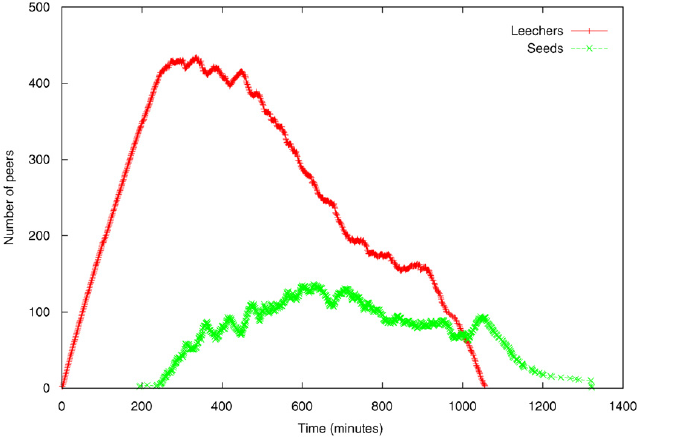
\includegraphics[width=15cm]{experiment}} \caption{\label{fig:experiment}
 نمایش روند تغییر تعداد مالکان فایل (Seeds) در طول زمان
 } \end{figure}

\subsection{نتایج پیاده‌سازی}
مدل پیاده‌سازی شده با توجه به محدودیت زمانی، تفاوت‌های زیادی با یک بیت‌تورنت واقعی دارد. اگرچه مکانیزم اصلی آن مشابه فرایند بیت‌تورنت است. برای نمایش نتیجه اجرا به‌جای نمودار پیشنهادی مقاله از نمودار میزان دریافت و ارسال میان کلاینت‌ها استفاده می‌کنیم تا مشخص شود چقدر همکاری که مد نظر پروتکل بیت‌تورنت بوده، محقق شده است.

در شکل \ref{fig:torrent} مشاهده می‌کنیم که دریافت و ارسال قطعات فایل اصلا در کلاینت خاصی متمرکز نشده است. این شکل حاصل به اشتراک گذاشتن یک فایل ۱۰۰ قطعه‌ای میان ۱۰ کلاینت است. در هنگام شروع تنها یک کلاینت مالک فایل است و پس از اجرا همه صاحب فایل شده‌اند. در طول زمان اجرا هر کلاینت قطعه‌هایی را که دریافت کرده مشخص می‌کند تا معلوم شود چقدر در کل مجموعه همکاری داشته‌ایم. در این شکل، هرچه خط میان دو کلاینت تیره‌تر باشد، نشان می‌دهد که آن دو با هم بیشتر همکاری کرده‌اند.
 
\begin{figure} \centerline{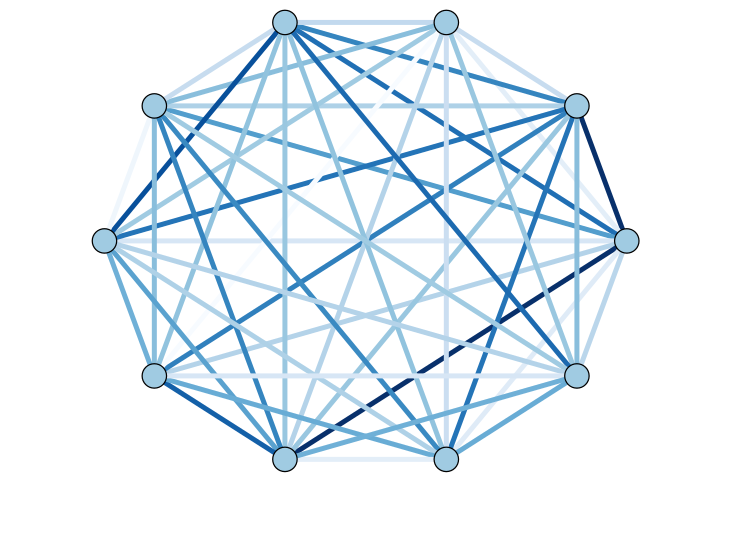
\includegraphics[width=13cm]{torrent}} \caption{\label{fig:torrent}
میزان همکاری میان کلاینت‌ها در توزیع یک فایل
 } \end{figure}

اگر قرار بود از روش مرسوم کلاینت-سرور برای توزیع فایل میان کاربران استفاده کنیم، نتیجه شبیه به شکل \ref{fig:server} می‌شد. همانطور که مشخص است در این شکل همه‌ی بار توزیع فایل بر دوش یک سرور قرار گرفته و این سرور عامل محدود کننده‌ی کارایی شبکه است.

\begin{figure} \centerline{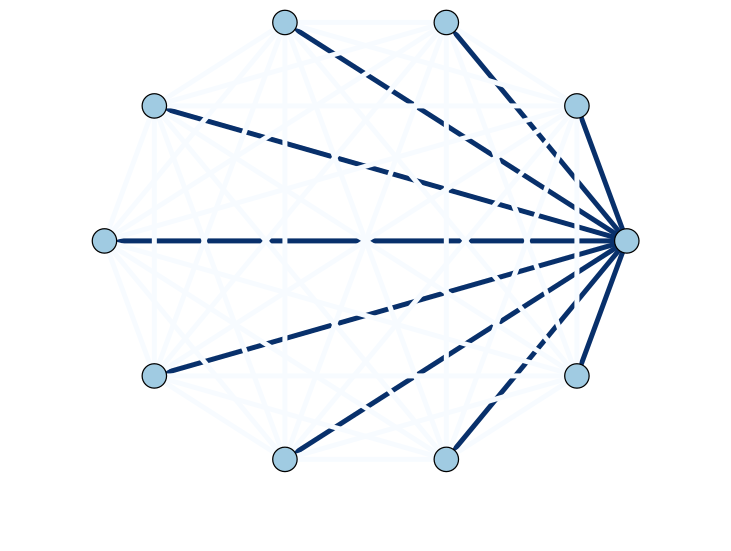
\includegraphics[width=13cm]{server}} \caption{\label{fig:server}
استفاده از مدل کلاینت-سرور برای توزیع یک فایل
 } \end{figure}

\renewcommand*{\refname}{\section{منابع}}
\begin{thebibliography}{9}
\begin{latin}

\bibitem{mas-torrent}
E. Costa-Montenegro, J. Burguillo-Rial, F. Gil-Castiñeira, and F. González-Castaño, “Implementation and analysis of the BitTorrent protocol with a multi-agent model,” Journal of Network and Computer Applications, vol. 34, no. 1, pp. 368–383, 2011.

\bibitem{wooldridge}
M. Wooldridge and N. R. Jennings, “Intelligent agents: Theory and practice,” Knowledge engineering review, vol. 10, no. 2, pp. 115–152, 1995.

\bibitem{spade}
M. E. Gregori, J. P. Cámara, and G. A. Bada, “A jabber-based multi-agent system platform,” in Proceedings of the fifth international joint conference on Autonomous agents and multiagent systems, 2006, pp. 1282–1284.

\end{latin}
\end{thebibliography}

\end{document}
